\documentclass[UTF8,a4paper,11pt]{ctexart}

% ── Page geometry ──
\usepackage[margin=2.2cm,top=2.5cm,bottom=2.5cm]{geometry}

% ── Typography & math ──
\usepackage{fontspec}
\usepackage{amsmath,amssymb}
\usepackage{setspace}
\setstretch{1.25}

% ── Graphics ──
\usepackage{tikz}
\usetikzlibrary{arrows.meta,calc}

% ── Colors ──
\usepackage{xcolor}
\definecolor{accent}{HTML}{1a73e8}
\definecolor{darkgray}{HTML}{333333}
\definecolor{lightgray}{HTML}{f5f5f5}
\definecolor{notebg}{HTML}{e8f0fe}
\definecolor{warnbg}{HTML}{fef7e0}
\definecolor{calcbg}{HTML}{e6f4ea}
\definecolor{calcframe}{HTML}{188038}

% ── Links ──
\usepackage{hyperref}
\hypersetup{colorlinks=true,linkcolor=accent,urlcolor=accent}

% ── Layout ──
\usepackage{enumitem}
\setlist[itemize]{leftmargin=1.8em,itemsep=2pt}
\setlist[enumerate]{leftmargin=1.8em,itemsep=2pt}
\usepackage{booktabs}
\usepackage{tcolorbox}
\usepackage{titlesec}
\usepackage{fancyhdr}
\usepackage{lastpage}

% ── Header/Footer ──
\pagestyle{fancy}
\fancyhf{}
\fancyhead[L]{\small\textcolor{darkgray}{文科生的微积分 · 七天讲义}}
\fancyhead[R]{\small\textcolor{darkgray}{从第一性原理理解变化与累积}}
\fancyfoot[C]{\small\textcolor{darkgray}{\thepage\ / \pageref{LastPage}}}
\renewcommand{\headrulewidth}{0.4pt}

% ── Section styling ──
\titleformat{\section}
  {\Large\bfseries\color{accent}}
  {\thesection}{1em}{}
\titleformat{\subsection}
  {\large\bfseries\color{darkgray}}
  {\thesubsection}{1em}{}

% ── Custom boxes ──
\newtcolorbox{keyconcept}[1][]{
  colback=notebg, colframe=accent,
  fonttitle=\bfseries, boxrule=0.5pt,
  left=8pt, right=8pt, top=6pt, bottom=6pt, title={#1}}
\newtcolorbox{exercise}[1][]{
  colback=warnbg, colframe=orange,
  fonttitle=\bfseries, boxrule=0.5pt,
  left=8pt, right=8pt, top=6pt, bottom=6pt, title={#1}}
\newtcolorbox{calcbox}[1][]{
  colback=calcbg, colframe=calcframe,
  fonttitle=\bfseries, boxrule=0.5pt,
  left=8pt, right=8pt, top=6pt, bottom=6pt, title={#1}}

\newcommand{\daytitle}[2]{%
  \section*{#1\quad #2}%
  \addcontentsline{toc}{section}{#1\quad #2}}
\newcommand{\unitmeta}[3]{% 优先级 / 难度 / 用时（调用处写全字样，便于源码审查）
  \noindent\textcolor{darkgray}{\small #1 ｜ #2 ｜ #3}\par\smallskip}

\begin{document}

% ═══ 封面 ═══
\begin{center}
  \vspace*{1.8cm}
  {\Huge\bfseries\color{accent} 文科生的微积分}\\[0.4cm]
  {\LARGE 七天讲义}\\[1.1cm]
  {\large 写给心理学、经济学、社会学、语言学……的文科生：\\
   从第一性原理理解“变化”与“累积”}\\[0.6cm]
  {\small\textcolor{darkgray}{主教材：《普林斯顿微积分读本》（Adrian Banner，人民邮电出版社中译本）}}\\[0.2cm]
  {\small\textcolor{darkgray}{配套开放资源：OpenStax Calculus Vol.1 · Paul's Online Math Notes · 3Blue1Brown}}\\[0.3cm]
  {\small\textcolor{darkgray}{\today}}
  \vfill
  {\small 每天 60–90 分钟：先读讲解，再合上讲义把概念讲出来，最后做自测。}
\end{center}
\newpage

\tableofcontents
\newpage

% ═══ 开始前 ═══
\section*{开始前：这本讲义在做什么}
\addcontentsline{toc}{section}{开始前：这本讲义在做什么}

微积分整门课，其实只回答两个问题：

\begin{enumerate}
  \item \textbf{某一点上，变化有多快？}→ 微分（求导）：变化率、斜率、边际量。
  \item \textbf{无数微小的变化累积起来，总量是多少？}→ 积分：面积、累积量、总量。
\end{enumerate}

而\textbf{微积分基本定理}说：这两个操作互为逆运算。七天就是把这一句话展开。

\textbf{为什么文科生要学这个}：你的专业课里到处都是它的影子——

\begin{itemize}
  \item 心理学：韦伯–费希纳定律 $S=k\ln(I/I_0)$、学习曲线、遗忘曲线（第 1、4、7 天）；
  \item 经济学：边际效用、边际成本——“边际”就是导数（第 3、5 天）；连续复利引出 $e$（第 2 天）；
  \item 社会学/政治学：洛伦兹曲线与基尼系数——不平等是用积分面积量出来的（第 6 天）；
  \item 一切实证研究：回归用最小二乘、估计用最大似然、概率是曲线下面积（第 5、6、7 天）。
\end{itemize}

\begin{keyconcept}[七天要带走的三样工具]
\begin{itemize}
  \item \textbf{极限的眼光}：不问“到达了没有”，只问“无限靠近时去哪儿”。这是微积分和高中数学最大的分水岭。
  \item \textbf{变化率}（导数）：瞬时变化有多快。斜率、速度、边际量，全是同一件事的换装。
  \item \textbf{微积分基本定理}：微分和积分互为逆运算——算“无限求和”变成“找原函数做两次减法”。
\end{itemize}
\end{keyconcept}

\textbf{七天的依赖关系图}（箭头 = 前提关系；粗线 = 必看主线）：

\begin{center}
\begin{tikzpicture}[
  day/.style={draw=accent, fill=notebg, rounded corners=3pt,
              minimum width=2.9cm, minimum height=0.9cm,
              font=\small, align=center},
  main/.style={-{Stealth[length=2.5mm]}, very thick, accent},
  sub/.style={-{Stealth[length=2mm]}, thin, darkgray}]
  \node[day] (d1) at (0,0) {第 1 天\\函数};
  \node[day] (d2) at (3.4,0) {第 2 天\\极限};
  \node[day] (d3) at (6.8,0) {第 3 天\\导数};
  \node[day] (d4) at (10.2,0) {第 4 天\\求导法则};
  \node[day] (d5) at (10.2,-1.8) {第 5 天\\导数应用};
  \node[day] (d6) at (3.4,-1.8) {第 6 天\\积分};
  \node[day] (d7) at (6.8,-1.8) {第 7 天\\基本定理};
  \draw[main] (d1) -- (d2);
  \draw[main] (d2) -- (d3);
  \draw[main] (d3) -- (d4);
  \draw[main] (d4) -- (d5);
  \draw[main] (d6) -- (d7);
  \draw[sub] (d3) -- (d6);
  \draw[sub] (d2) -- (d6);
  \draw[sub] (d1) to[bend right=18] (d6);
\end{tikzpicture}
\end{center}

主线 $1\to2\to3\to4\to5$ 是微分半边，$3\to6\to7$ 是积分半边；第 7 天把两半焊起来。时间紧的话第 5 天可只读前半、第 4 天的商法则可跳过。

\begin{calcbox}[边界声明]
\begin{itemize}
  \item \textbf{覆盖}：一元函数微积分主干——函数与图像、极限与连续、导数与求导法则、导数应用（极值/凹凸/最优化）、不定积分与定积分、换元法、微积分基本定理。对应文科高等数学/经管类微积分一学期课程的核心考试范围。
  \item \textbf{不覆盖}：级数与泰勒展开、多元微积分（只口头提一句偏导）、微分方程、严格的 $\varepsilon$–$\delta$ 证明。这些列入书末“后续学习指引”。
  \item \textbf{目标}：建立直觉 + 抓住主干 + 会算基础题，不追求刷题量与计算速度。
\end{itemize}
\end{calcbox}

\textbf{读者预设}：你会高中文科数学（基本函数的图像、幂运算、简单三角），但\textbf{从没见过}极限和导数。所有新概念从零讲起。

\textbf{每天的学习流程}（60–90 分钟）：
\begin{enumerate}
  \item 读当天的讲解，重点看“为什么这样定义”，不要背结论；
  \item 合上讲义，把当天的核心概念\textbf{讲给别人听}（或讲给自己听），卡壳的地方就是没懂的地方；
  \item 做“今日自测”，对照书末的参考答案（答案给思路要点，不只给结果）。
\end{enumerate}

\newpage

% ═══ 第 1 天 ═══
\daytitle{第 1 天}{函数：把世界翻译成“输入 → 输出”}
\unitmeta{优先级：【必看】}{难度：$\bigstar$}{用时：约 75 分钟}

\textbf{核心问题}：为什么文科的定律（感受、财富、遗忘）最后都写成了函数？

\subsection*{1.1 函数是“对应规则”，不是“算式”}

函数 $f$ 只做一件事：给一个输入 $x$，返回唯一确定的输出 $f(x)$。它不需要“公式”——一张对照表、一条曲线、一句规则都是函数。公式只是最方便书写的那一种。

为什么文科生绕不开它？因为各学科的“定律”几乎都是函数声明：

\begin{itemize}
  \item 心理学·韦伯–费希纳定律：主观感受强度是物理刺激的对数函数 $S = k\ln(I/I_0)$（$I_0$ 是刚好能感觉到的最小刺激，叫绝对阈限）；
  \item 心理学·史蒂文斯幂定律：$\psi = kI^{a}$，$a$ 因感觉通道而异（响度约 $0.67$，电击约 $3.5$）；
  \item 经济学·复利：本金 $P$、年利率 $r$、$t$ 年后变成 $A = P(1+r)^{t}$——指数函数；
  \item 人口学：指数增长 $N = N_0 e^{rt}$。
\end{itemize}

这三类函数——\textbf{对数、幂、指数}——就是文科世界里最常出现的三种“增长性格”：对数越来越慢，幂函数居中，指数越来越快。

\subsection*{1.2 三种增长性格，一张图}

\begin{center}
\begin{tikzpicture}[scale=0.62]
  % 坐标轴
  \draw[-{Stealth}] (0,0) -- (10.6,0) node[below left]{\small 刺激 / 时间 $x$};
  \draw[-{Stealth}] (0,0) -- (0,4.8) node[below left]{\small $f(x)$};
  % 对数 ln(1+x)/ln(11)*4：x=0→0, x=10→4
  \draw[very thick, accent] plot[domain=0:10, samples=60] (\x,{4*ln(1+\x)/ln(11)});
  \node[accent, font=\small] at (9.2,4.15) {$\ln$：越来越慢};
  % 幂 x^0.5：x=0→0, x=10→√10/√10*3.4
  \draw[very thick, calcframe] plot[domain=0:10, samples=60] (\x,{3.4*sqrt(\x)/sqrt(10)});
  \node[calcframe, font=\small] at (7.6,1.6) {$x^{0.5}$：居中};
  % 指数 e^{x/3.5}-1 归一：x=10→ e^{2.857}-1≈16.4 → 缩放 4.4/16.4
  \draw[very thick, orange] plot[domain=0:10, samples=60] (\x,{4.4*(exp(\x/3.5)-1)/(exp(10/3.5)-1)});
  \node[orange, font=\small] at (8.2,3.15) {$e^{x}$：越来越快};
\end{tikzpicture}
\end{center}

三条曲线都经过 $(0,0)$，右端对齐在同一高度——差别全在\textbf{途中}：对数在前半程冲得最猛、后劲衰竭；指数相反。这就是“增长性格”的含义。

\begin{keyconcept}[为什么“感受”是对数的？]
韦伯定律说：能察觉的最小差别 $\Delta I$ 与当前刺激 $I$ 成比例，即 $\Delta I / I = $ 常数。提 1 kg 重物时多放 10 g 你能察觉；提 10 kg 时要多放 100 g 才察觉——同样的 $\Delta I$，刺激越大越“钝”。把这个比例关系累积起来（第 6 天会说“累积”就是积分），得到的正是对数函数：$S = k\ln(I/I_0)$。\textbf{对数不是数学家发明的记号，是“敏感度随基数递减”这条经验的必然形状。}Bernoulli 在 1738 年用同样的 $u(x)=\log x$ 描述财富的主观价值（边际效用递减）——心理物理学和决策科学共享同一条曲线。
\end{keyconcept}

\subsection*{1.3 读图三件套：定义域、单调性、增长性格}

拿到一个函数，文科生只需要三个问题：

\begin{enumerate}
  \item \textbf{定义域}：哪些输入合法？$\ln x$ 只吃 $x>0$；$\sqrt{x}$ 不吃负数。
  \item \textbf{单调性}：上升还是下降？遗忘曲线单调下降，学习曲线（成绩–练习）单调上升。
  \item \textbf{增长性格}：越来越快还是越来越慢？这决定了曲线的弯曲方向——第 5 天的“凹凸”就是把它精确化。
\end{enumerate}

\begin{calcbox}[易错点与失效边界]
\begin{itemize}
  \item \textbf{定义域先行}：$\ln x$、$\sqrt{x}$ 的输入必须为正（或非负）；列式前先问“这个输入合法吗”。
  \item “增长越来越慢”$\neq$“有上界”：$\ln x$ 慢但无界，渐近线（如学习曲线的下限）才是真上/下限。
  \item 指数增长（$2^{x}$）最终超过一切幂增长（$x^{2}$）——“底数动还是指数动”别搞反。
  \item 函数图像只是模型：真实数据（反应时、遗忘量）总有噪声，曲线是趋势不是预言。
\end{itemize}
\end{calcbox}

\begin{exercise}[今日自测]
\begin{enumerate}
  \item 某记忆实验测得遗忘量 $R(t)=e^{-t/2}$（$t$ 以天计）。说出它的单调性与增长性格，并算出 $R(0)$、$R(2)$（保留两位小数）。
  \item 韦伯–费希纳定律 $S=k\ln(I/I_0)$ 中，刺激从 $I_0$ 增大到 $10I_0$、再从 $10I_0$ 增大到 $100I_0$，两次感受增量一样大吗？用对数性质说明。
  \item 判断：因为 $\ln x$ 增长越来越慢，所以 $\ln x$ 有上界（涨到某个值就不再涨）。对吗？
  \item 向一个没学过高等数学的同学解释：为什么“感觉”适合用对数、“病毒传播初期”适合用指数？各用一句日常类比。
\end{enumerate}
\end{exercise}

\newpage

% ═══ 第 2 天 ═══
\daytitle{第 2 天}{极限：只问趋势，不问到达}
\unitmeta{优先级：【必看】}{难度：$\bigstar\bigstar\bigstar$}{用时：约 85 分钟}

\textbf{核心问题}：一个量“无限靠近”某个值却永远不到达，这话怎么变成精确的数学？

\subsection*{2.1 极限的直觉：终点不重要，路线才重要}

复利实验：本金 1 元，年利率 100\%，一年结算 1 次得 $2$ 元；半年结算 1 次（每次 50\%）得 $1.5^2=2.25$ 元；每月结算得 $(1+\tfrac{1}{12})^{12}\approx 2.613$ 元；每天结算得 $(1+\tfrac{1}{365})^{365}\approx 2.7146$ 元。结算越来越频繁，本息和\textbf{靠近}一个固定的数——但从不超过它：

\[
  \lim_{n\to\infty}\Bigl(1+\frac{1}{n}\Bigr)^{n} = e \approx 2.71828\ldots
\]

这就是自然常数 $e$ 的定义（“连续复利”）。注意两件事：第一，$n$ 永远到不了“无穷大”，我们只是问\textbf{趋势}；第二，极限值 $e$ 不是任何一步算出来的结果，而是整条路线指向的目的地。记法 $\lim_{x\to a}f(x)=L$ 读作：$x$ 无限靠近 $a$ 时，$f(x)$ 无限靠近 $L$。

\begin{keyconcept}[极限为什么不定义为“代入”？]
代入要求函数在 $a$ 点有定义且“正常”，但微积分最关心的恰恰是函数\textbf{没定义}的点：第 3 天的导数定义里，$h=0$ 处函数根本不存在（$0/0$），可它的极限存在且意义重大。把极限定义为“代入的结果”，等于在门口就把导数枪毙了。所以极限只问“靠近时去哪儿”，不问“到了没有”——这是被设计出来的定义，为的是能谈论那些“差一点就到达”的点。
\end{keyconcept}

\subsection*{2.2 计算极限的三件事（考试 90\% 的题）}

\begin{enumerate}
  \item \textbf{能代入就代入}：$\lim\limits_{x\to 2}(x^2+1)=5$。函数在该点“正常”（连续，见下）时，极限就是函数值。
  \item \textbf{代入出 $\tfrac{0}{0}$：先化简再代入}。例：
  \[
    \lim_{x\to 1}\frac{x^2-1}{x-1}
    =\lim_{x\to 1}\frac{(x-1)(x+1)}{x-1}
    =\lim_{x\to 1}(x+1)=2 .
  \]
  $x=1$ 处函数无定义，但极限是 $2$——“无限靠近 1 时，值无限靠近 2”。
  \item \textbf{$x\to\infty$ 的有理函数：只看最高次项}。
  \[
    \lim_{x\to\infty}\frac{3x^2+x}{5x^2-7}=\frac{3}{5},
    \qquad\text{因为低次项在无穷大面前可以忽略。}
  \]
\end{enumerate}

\subsection*{2.3 连续：图像“不断开”}

直觉定义：$f$ 在 $a$ 点连续 $\iff$ 极限值 $=$ 函数值，即 $\lim_{x\to a}f(x)=f(a)$。连续函数的图像一笔画成、没有跳断。为什么它有用？因为连续函数允许你“从中间值的存在性”推理：如果温度从 10 ℃ 连续升到 20 ℃，那必然经过 15 ℃（介值定理）——社会统计里“收入分布连续变化”这类论证背后都是它。

\begin{calcbox}[易错点与失效边界]
\begin{itemize}
  \item \textbf{极限存在 $\neq$ 函数在该点有定义}（2.2 第 2 条就是例子）。反过来，函数有定义也不保证极限存在（在该点乱跳就不行）。
  \item \textbf{左右极限不等}时极限不存在：$\lim_{x\to 0}\tfrac{|x|}{x}$，从右边靠近是 $+1$，从左边是 $-1$——两边谈不拢，极限不存在。
  \item “只看最高次项”只对 $x\to\infty$ 的\textbf{有理函数}成立；$x\to 0$ 时恰恰是低次项说了算。
  \item $\tfrac{0}{0}$ 不是答案，是“需要化简”的信号灯；$\tfrac{1}{0}$ 型则通常意味着极限不存在（发散到无穷）。
\end{itemize}
\end{calcbox}

\begin{exercise}[今日自测]
\begin{enumerate}
  \item 计算：$\lim\limits_{x\to 3}\dfrac{x^2-9}{x-3}$；$\lim\limits_{x\to\infty}\dfrac{2x^3-x}{4x^3+7}$。
  \item 学习曲线 $RT(N)=0.4+0.6\cdot N^{-0.5}$（$N$ 为练习次数，$RT$ 为反应时，单位秒）。练习无限增多时，反应时趋向多少？这个极限值在心理学上叫什么？
  \item 辨析：$\lim\limits_{x\to 0}(1+x)^{1/x}$ 存在吗？它和今天的哪个例子本质相同？
  \item 向同学解释“极限只问趋势不问到达”，用复利或追公交车的例子，不超过三句话。
\end{enumerate}
\end{exercise}

\newpage

% ═══ 第 3 天 ═══
\daytitle{第 3 天}{导数：把“变化有多快”变成一个数}
\unitmeta{优先级：【必看】}{难度：$\bigstar\bigstar\bigstar$}{用时：约 90 分钟}

\textbf{核心问题}：“现在这一瞬间”变化有多快——没有时间段，怎么算变化率？

\subsection*{3.1 从平均到瞬时：极限的第一次实战}

平均变化率好算：反应时从第 1 天的 0.9 s 降到第 5 天的 0.5 s，平均每天降 0.1 s。但“第 3 天\textbf{当天}进步有多快”？时间段缩成一个点，$\tfrac{\Delta y}{\Delta x}$ 变成 $\tfrac{0}{0}$——昨天学的极限此刻派上用场：

\[
  f'(x)=\lim_{h\to 0}\frac{f(x+h)-f(x)}{h}
\]

$h$ 是时间段的宽度。$h$ 越小，割线越贴着曲线旋转；$h\to 0$ 的极限位置叫\textbf{切线}，切线的斜率就是导数。下图是 $y=x^2$ 在 $x=1$ 处的真实情形：

\begin{center}
\begin{tikzpicture}[scale=1.05]
  \draw[-{Stealth}] (-0.4,0) -- (3.1,0) node[below left]{\small $x$};
  \draw[-{Stealth}] (0,-1.4) -- (0,4.6) node[below left]{\small $y$};
  % 抛物线 y=x^2
  \draw[very thick, darkgray] plot[domain=-0.3:2.1, samples=60] (\x,{\x*\x});
  \node[darkgray, font=\small] at (2.35,4.0) {$y=x^2$};
  % 割线：过 (1,1) 与 (2,4)，斜率 3 → y=3x-2
  \draw[thick, orange, dashed] plot[domain=0.45:2.35] (\x,{3*\x-2});
  \node[orange, font=\small] at (2.52,2.6) {割线：斜率 $3$};
  % 切线：x=1 处斜率 2 → y=2x-1
  \draw[very thick, accent] plot[domain=0.0:2.0] (\x,{2*\x-1});
  \node[accent, font=\small] at (0.62,2.45) {切线：斜率 $2$};
  % 点
  \fill (1,1) circle (1.6pt) node[below right=2pt]{\small $(1,1)$};
  \fill (2,4) circle (1.6pt) node[right]{\small $(2,4)$};
  \draw[thin, darkgray] (1,0) node[below]{\small $1$} -- (1,1);
  \draw[thin, darkgray] (2,0) node[below]{\small $2$} -- (2,4);
\end{tikzpicture}
\end{center}

割线取 $h=1$（从 $x=1$ 到 $x=2$）：斜率 $=\tfrac{4-1}{2-1}=3$。$h$ 缩小，割线斜率趋于 $2$——这就是 $f'(1)=2$。图是按解析式 $y=3x-2$（割线）与 $y=2x-1$（切线）画的，切线与抛物线只在 $(1,1)$ 相触，你可以拿尺子验证。

\begin{keyconcept}[“边际”就是导数]
经济学把“多生产一单位，成本增加多少”叫边际成本——那是离散的说法。把产量看成连续变量，边际成本 $=$ 成本函数的\textbf{导数}；边际效用 $=$ 效用函数的导数。Bernoulli 的对数效用 $u(x)=\log x$ 的边际效用是 $u'(x)=1/x$：财富越多，每多一元带来的效用增量越小。你在经济学课背的“边际量递减/递增”，翻译成微积分就是“导数在变小/变大”。
\end{keyconcept}

\subsection*{3.2 用定义算一次（就这一次）}

按定义求 $f(x)=x^2$ 的导数：

\[
  f'(x)=\lim_{h\to0}\frac{(x+h)^2-x^2}{h}
       =\lim_{h\to0}\frac{2xh+h^2}{h}
       =\lim_{h\to0}(2x+h)=2x .
\]

三步看门道：展开（分子出现公因子 $h$）→ 约分（$\tfrac{0}{0}$ 消失）→ 代入 $h=0$（极限的“三件事”第 2 条）。结论是 $(x^2)'=2x$——下一天你会发现它在公式表第一行。\textbf{定义用来理解，公式表用来干活}，从此以后再遇到求导，查表即可。

\begin{calcbox}[易错点与失效边界]
\begin{itemize}
  \item \textbf{导数是函数，不是单个数}：$f'(x)=2x$ 在每一点取值不同（$f'(1)=2$，$f'(3)=6$）。
  \item \textbf{切线斜率 $\neq$ 割线斜率}：$h$ 不取极限，得到的只是平均变化率。
  \item \textbf{尖点处导数不存在}：$y=|x|$ 在 $x=0$ 左边斜率 $-1$、右边 $+1$，割线极限谈不拢——图像光滑才谈得上切线。
  \item 可导必连续，连续未必可导（$|x|$ 就是连续但尖点不可导的例子）。
\end{itemize}
\end{calcbox}

\begin{exercise}[今日自测]
\begin{enumerate}
  \item 用导数定义（展开→约分→代入）求 $f(x)=x^2+3x$ 的导数。
  \item 成本函数 $C(q)=q^2$（千元），$q$ 为产量（百件）。$f'(q)=2q$：$q=5$ 时边际成本是多少？$q=10$ 时呢？这说明了什么？
  \item 判断：函数在某点连续，则该点一定有导数。对吗？给理由或反例。
  \item 向学经济学的朋友解释“边际成本是导数”，要求用上“多生产一单位”和“极限”两个词。
\end{enumerate}
\end{exercise}

\newpage

% ═══ 第 4 天 ═══
\daytitle{第 4 天}{求导法则：五分钟的表，半小时的链式}
\unitmeta{优先级：【必看】}{难度：$\bigstar\bigstar$}{用时：约 80 分钟}

\textbf{核心问题}：任何复杂函数都由简单函数拼成——能不能只记几条拼装规则，求出所有的导数？

\subsection*{4.1 基本公式表（背熟这五行）}

\begin{center}
\begin{tabular}{lll}
\toprule
$f(x)$ & $f'(x)$ & 一句话记忆 \\
\midrule
$x^{n}$ & $n\,x^{n-1}$ & 指数搬下来，指数减一 \\
$e^{x}$ & $e^{x}$ & 它自己是自己的导数 \\
$\ln x$ & $1/x$ & 感受的“边际”随刺激递减 \\
$\sin x$ & $\cos x$ & 相位领先四分之一周期 \\
$\cos x$ & $-\sin x$ & 注意负号 \\
\bottomrule
\end{tabular}
\end{center}

$e^x$ 那行不是巧合：$e$ 就是被定义为“让指数函数的导数等于自身”的底数（这正是第 2 天连续复利那个 $e$ 如此特殊的深层原因）。组合规则：和差的导数 $=$ 逐项求导；常数倍直接提出来：$(3x^2+5e^x)'=6x+5e^x$。

\subsection*{4.2 乘法与商法则（会用即可）}

\[
  (uv)'=u'v+uv',\qquad
  \Bigl(\frac{u}{v}\Bigr)'=\frac{u'v-uv'}{v^{2}} .
\]

例：$(x^2 e^x)' = 2x\cdot e^x + x^2\cdot e^x = e^x(2x+x^2)$。这两条\textbf{不用背推导}，但要知道它们不是“逐项求导”——$(uv)'\neq u'v'$，这是初学者最常见的错。

\subsection*{4.3 链式法则：本周最重要的公式}

复合函数 $f(g(x))$（外面包一层）的导数：

\[
  \bigl[f(g(x))\bigr]' = f'\bigl(g(x)\bigr)\cdot g'(x)
  \qquad\text{（外导 } \times \text{ 内导）}
\]

为什么合理？速度是“叠乘”的：$y$ 随 $u$ 变化的速度，乘上 $u$ 随 $x$ 变化的速度，就是 $y$ 随 $x$ 变化的速度——$\tfrac{dy}{dx}=\tfrac{dy}{du}\cdot\tfrac{du}{dx}$，链式法则正是这句话。

\begin{keyconcept}[链式法则实战：遗忘曲线降得有多快？]
现代常用的遗忘近似 $R(t)=e^{-t/S}$（$S$ 为记忆稳定性；此式出自 Woźniak 等 1995 年，艾宾浩斯 1885 年本人用的是对数型公式，见书末资料注）。外层 $e^{u}$ 的导数是自身，内层 $u=-t/S$ 的导数是 $-1/S$，于是
\[
  R'(t)=e^{-t/S}\cdot\Bigl(-\frac{1}{S}\Bigr)=-\frac{1}{S}R(t).
\]
\textbf{遗忘速度与当前剩余记忆量成正比}——剩得多忘得快，剩得少忘得慢。这就是“指数衰减”四个字的精确含义，也是复习间隔应该越拉越长的数学依据。
\end{keyconcept}

再练一个：$\bigl[\ln(3x^2+1)\bigr]'=\dfrac{1}{3x^2+1}\cdot 6x=\dfrac{6x}{3x^2+1}$。外层 $\ln$ 的导数是“分之一”，内层照常求导，乘起来。

\begin{calcbox}[易错点与失效边界]
\begin{itemize}
  \item 链式法则最常见的错是\textbf{忘乘内导}：$(e^{2x})'=2e^{2x}$，不是 $e^{2x}$。
  \item $(x^n)'=nx^{n-1}$ 只对\textbf{底数是 $x$、指数是常数}成立；$a^x$（指数是变量）的导数是 $a^x\ln a$，别套幂法则。
  \item 乘法法则别写成 $(uv)'=u'v'$；商法则分子是 $u'v-uv'$，顺序反了差一个负号。
  \item 对数对加法没有法则：$\ln(a+b)$ 不能拆。
\end{itemize}
\end{calcbox}

\begin{exercise}[今日自测]
\begin{enumerate}
  \item 求导：$f(x)=4x^3-2e^x+7$；$g(x)=x\cdot\ln x$。
  \item 求导（链式法则）：$h(x)=e^{-3x}$；$k(x)=\sqrt{2x^2+5}$（提示：$\sqrt{u}=u^{1/2}$）。
  \item 判断并改正：$\bigl[\sin(x^2)\bigr]'=\cos(x^2)$。
  \item 史蒂文斯幂定律 $\psi=kI^{a}$。求 $\psi'(I)$，并分别就 $a=0.67$（响度）与 $a=3.5$（电击）说明：刺激增大时，“每单位新增刺激带来的感受增量”如何变化？
\end{enumerate}
\end{exercise}

\newpage

% ═══ 第 5 天 ═══
\daytitle{第 5 天}{导数应用：单调、极值与“最好的点”}
\unitmeta{优先级：【必看】}{难度：$\bigstar\bigstar$}{用时：约 85 分钟}

\textbf{核心问题}：为什么“找最好”（最大效用、最小误差）最后都变成“令导数等于零”？

\subsection*{5.1 导数的符号 = 函数的方向}

$f'(x)>0$：函数在增；$f'(x)<0$：在减；$f'(x)=0$：切线水平——函数在这里“停了一下”，可能是山顶（极大值）、谷底（极小值），也可能只是歇脚（如 $y=x^3$ 在 $x=0$）。看一个构造好的例子 $y=x^3-3x$：

\begin{center}
\begin{tikzpicture}[scale=0.85]
  \draw[-{Stealth}] (-2.9,0) -- (2.9,0) node[below left]{\small $x$};
  \draw[-{Stealth}] (0,-2.9) -- (0,2.9) node[below left]{\small $y$};
  \draw[very thick, accent] plot[domain=-2.15:2.15, samples=80] (\x,{\x*\x*\x-3*\x});
  \node[accent, font=\small] at (2.0,2.5) {$y=x^3-3x$};
  \fill (-1,2) circle (1.8pt) node[above]{\small 极大 $(-1,2)$};
  \fill (1,-2) circle (1.8pt) node[below]{\small 极小 $(1,-2)$};
  % 水平切线提示
  \draw[thin, orange, dashed] (-1.6,2) -- (-0.4,2);
  \draw[thin, orange, dashed] (0.4,-2) -- (1.6,-2);
  \foreach \x in {-2,-1,1,2} \draw[thin, darkgray] (\x,0) node[below]{\small $\x$} -- (\x,0.06);
\end{tikzpicture}
\end{center}

验证：$y'=3x^2-3=3(x-1)(x+1)$，零点恰为 $x=\pm1$；代回原式得 $y(\pm1)=\mp2$，与图中标注一致。$x<-1$ 时 $y'>0$（升），$-1<x<1$ 时 $y'<0$（降），$x>1$ 时 $y'>0$（升）——符号表就是图像的“文字版”。

\subsection*{5.2 求极值/最值三步}

\begin{enumerate}
  \item \textbf{求导}，解 $f'(x)=0$，得驻点；
  \item \textbf{判断}：看 $f'$ 在驻点两侧是否变号（左正右负 $=$ 极大，左负右正 $=$ 极小）；或看二阶导 $f''$ 在该点的正负（$f''>0$ 谷底，$f''<0$ 山顶）；
  \item 求\textbf{最值}时，把驻点和区间端点的函数值一起比较，取最大/最小。
\end{enumerate}

二阶导 $f''$ 还有独立含义：它刻画\textbf{弯曲方向}。$f''>0$ 凹向上（像碗），$f''<0$ 凹向下（像伞）。“增长越来越慢”（对数）就是 $f'>0$ 且 $f''<0$；“越来越快”（指数）是 $f'>0$ 且 $f''>0$。第 1 天的“增长性格”，现在有了精确说法。

\subsection*{5.3 文科研究的发动机：最小二乘与最大似然}

\begin{keyconcept}[为什么回归和估计都在“求导 = 0”？]
最小二乘法：给数据点 $(x_i,y_i)$ 配直线 $y=mx+b$，总误差 $E(m,b)=\sum\bigl(y_i-mx_i-b\bigr)^2$。$E$ 是 $m$、$b$ 的开口向上的“碗”，碗底就是误差最小点；碗底的特征是每个方向的导数都为 $0$——对 $m$、$b$ 分别求导（多元时叫偏导，每次只动一个变量）并令其为 $0$，解出的正是回归系数公式。\textbf{“最小二乘”四个字里没有导数，但它的求解动作就是第 5.2 节那三步。}最大似然估计同理：似然函数（或对数似然 $\ell(\theta)$）取最大的参数 $\theta$，候选点满足 $\ell'(\theta)=0$。你以后在统计软件里点一下“回归”，背后跑的就是这一套。
\end{keyconcept}

\begin{calcbox}[易错点与失效边界]
\begin{itemize}
  \item $f'(x)=0$ 是极值的\textbf{必要非充分}条件：$y=x^3$ 在 $x=0$ 处 $y'=0$，但两侧都是增，没有极值。必须做第 2 步判断。
  \item 极值（局部高低）$\neq$ 最值（全局高低）：区间端点不参与 $f'=0$ 的筛选，却可能是最值。
  \item $f''=0$ 不一定是拐点（凹凸切换点），还要看 $f''$ 是否变号。
  \item 最小二乘的“求导 = 0”能给出最小值，前提是该问题确实只有唯一的“碗底”——异常值很多时最小二乘本身会失真，那是方法论的失效边界，不是微积分的错。
\end{itemize}
\end{calcbox}

\begin{exercise}[今日自测]
\begin{enumerate}
  \item 求 $f(x)=x^3-12x$ 的全部极值点，并判断极大还是极小（用一阶导符号或二阶导均可）。
  \item 某商品利润（百元）$P(x)=-2x^2+40x-150$，$x$ 为广告投入（千元）。广告投入多少时利润最大？最大利润是多少？
  \item 判断：若 $f'(a)=0$ 且 $f''(a)>0$，则 $f$ 在 $a$ 处取得极小值。对吗？
  \item 向同学解释“为什么最小二乘法要求导”，提示从“碗底有什么几何特征”说起。
\end{enumerate}
\end{exercise}

\newpage

% ═══ 第 6 天 ═══
\daytitle{第 6 天}{积分：把无数小份累积成总量}
\unitmeta{优先级：【必看】}{难度：$\bigstar\bigstar\bigstar$}{用时：约 90 分钟}

\textbf{核心问题}：知道每一小份有多少，怎么把它们“加无穷多次”得出总量？

\subsection*{6.1 面积问题：无穷求和的入口}

曲线 $y=f(x)$ 下方、从 $a$ 到 $b$ 的面积怎么算？切蛋糕：把区间切成 $n$ 个窄条，每条宽 $\Delta x$，高近似为 $f(x_i)$，面积 $\approx \sum f(x_i)\,\Delta x$；条越窄越准，$n\to\infty$ 时的极限就是\textbf{定积分}：

\[
  \int_a^b f(x)\,dx=\lim_{n\to\infty}\sum_{i=1}^{n}f(x_i)\,\Delta x
\]

下图是 $y=x^2$ 在 $[0,2]$ 上用 4 个矩形逼近（每块宽 $0.5$，高取右端点函数值）：

\begin{center}
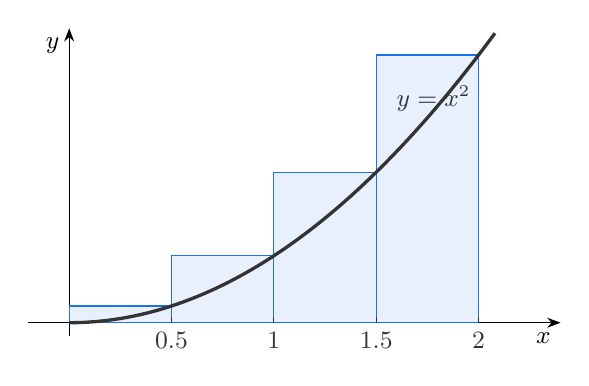
\begin{tikzpicture}[x=2.6cm,y=0.85cm]
  \draw[-{Stealth}] (-0.2,0) -- (2.4,0) node[below left]{\small $x$};
  \draw[-{Stealth}] (0,-0.2) -- (0,4.4) node[below left]{\small $y$};
  % 4 rectangles width 0.5, right-endpoint heights (0.5,1,1.5,2)^2 = 0.25,1,2.25,4
  \foreach \xa/\h in {0/0.25, 0.5/1, 1/2.25, 1.5/4}{
    \draw[fill=notebg, draw=accent] (\xa,0) rectangle ({\xa+0.5},\h);}
  \draw[very thick, darkgray] plot[domain=0:2.08, samples=60] (\x,{\x*\x});
  \node[darkgray, font=\small] at (1.78,3.35) {$y=x^2$};
  \foreach \x in {0.5,1,1.5,2} \draw[thin, darkgray] (\x,0) node[below]{\small $\x$} -- (\x,0.08);
\end{tikzpicture}
\end{center}

矩形总面积 $=0.5\times(0.25+1+2.25+4)=3.75$，比真实面积偏大（矩形冒出了曲线之上）。条数加倍，逼近更好；明天的基本定理会给出精确值 $\tfrac{8}{3}\approx2.67$。\textbf{定积分是“求和的极限”}——它和第 2 天的极限、第 3 天的导数是同一个思想家族。

经济学里同一个思想换个名字：边际成本曲线的积分 $=$ 总成本；社会学里，洛伦兹曲线与对角线之间的\textbf{面积}（占三角形总面积的比例）就是基尼系数——“不平等”是被积分量出来的。

\subsection*{6.2 不定积分：求导的反操作}

$\int f(x)\,dx$ 问的是：哪个函数求导等于 $f(x)$？答案叫\textbf{原函数}，且不唯一（差一个常数），所以永远带 $+C$：

\[
  \int x^{n}\,dx=\frac{x^{n+1}}{n+1}+C\ (n\neq-1),\quad
  \int\frac{1}{x}\,dx=\ln|x|+C,\quad
  \int e^{x}\,dx=e^{x}+C .
\]

公式表就是第 4 天导数表\textbf{倒着读}。验证永远是同一个动作：对结果求导，看是否回到被积函数。

\subsection*{6.3 换元法：链式法则的逆用}

看到复合结构，把内层整体换成 $u$：

\[
  \int 2x\,e^{x^{2}}dx\ \xrightarrow{u=x^{2},\ du=2x\,dx}\ \int e^{u}\,du=e^{u}+C=e^{x^{2}}+C .
\]

识别信号：被积函数里\textbf{同时出现}某表达式和它的导数（$x^2$ 与 $2x$）。文科考试掌握这一种技巧就够。

\begin{calcbox}[易错点与失效边界]
\begin{itemize}
  \item \textbf{丢 $+C$}：不定积分的结果是一族函数，漏写常数是考试必扣分点。
  \item $\int x^{-1}dx$ 不能套幂法则（分母会变成 $0$），它的答案是 $\ln|x|+C$——对数正是从这条裂缝里长出来的。
  \item 定积分是\textbf{数}（面积），不定积分是\textbf{函数族}（原函数），写法上只差上下限，含义完全不同。
  \item 换元后忘记把 $du$ 与 $dx$ 的关系代干净，是最常见的计算事故；定积分换元时上下限也要跟着换。
\end{itemize}
\end{calcbox}

\begin{exercise}[今日自测]
\begin{enumerate}
  \item 计算：$\displaystyle\int\bigl(3x^2+\tfrac{1}{x}\bigr)dx$；$\displaystyle\int e^{-t/2}dt$（提示：换元 $u=-t/2$）。
  \item 边际成本 $MC(q)=2q$（千元/百件）。总成本关于产量 $q$ 的函数是什么（设固定成本为 $10$ 千元）？
  \item 判断：$\displaystyle\int_a^b f(x)dx$ 的结果里应该写 $+C$。对吗？
  \item 用“窄条逼近”的语言，向同学解释为什么洛伦兹曲线和对角线之间的面积越小、社会越平等。
\end{enumerate}
\end{exercise}

\newpage

% ═══ 第 7 天 ═══
\daytitle{第 7 天}{微积分基本定理：把两半焊起来 + 一周总检验}
\unitmeta{优先级：【必看】}{难度：$\bigstar\bigstar\bigstar$}{用时：约 90 分钟}

\textbf{核心问题}：变化率和累积量，凭什么互为逆运算？

\subsection*{7.1 全课最高光的定理}

\textbf{微积分基本定理}：设 $F$ 是 $f$ 的任意一个原函数（$F'=f$），则

\[
  \int_a^b f(x)\,dx = F(b)-F(a) .
\]

左边是“无穷个窄条求和的极限”（第 6 天），右边只是“找一个原函数、做两次减法”。一个看似要无限操作的难题，被压缩成代数动作。例：昨天那个 $\int_0^2 x^2dx$，原函数 $F(x)=\tfrac{x^3}{3}$，于是

\[
  \int_0^2 x^2\,dx=\frac{2^3}{3}-\frac{0^3}{3}=\frac{8}{3}\approx 2.67 ,
\]

正是昨天矩形逼近（$3.75$ 偏大）所趋向的精确值。

为什么定理合理？把 $F(b)-F(a)$ 想成“总变化量”：它等于每一步微小变化 $dF$ 的累积；而每一步 $dF\approx F'(x)\,dx=f(x)\,dx$。总变化量 $=$ 变化率的累积——\textbf{导数拆开总量，积分拼回总量，两者互为逆运算}。整门课的结构一句话说清：

\begin{center}
\begin{tikzpicture}[
  box/.style={draw=accent, fill=notebg, rounded corners=3pt,
              minimum width=3.4cm, minimum height=1.0cm, font=\small, align=center},
  arr/.style={-{Stealth[length=2.5mm]}, very thick, accent}]
  \node[box] (f) at (0,0) {函数 $f(x)$\\（总量）};
  \node[box] (fp) at (7.2,0) {导数 $f'(x)$\\（变化率）};
  \draw[arr] (f) -- node[above, font=\small]{求导：拆开} (fp);
  \draw[arr] (fp) to[bend left=25] node[below, font=\small]{积分：拼回（$+C$）} (f);
\end{tikzpicture}
\end{center}

极限是语言（第 2 天），导数与积分是两种操作（第 3、6 天），基本定理是焊接点（今天）。

\subsection*{7.2 概率就是面积：通往统计的桥}

正态分布的密度曲线 $\varphi(x)=\tfrac{1}{\sqrt{2\pi}}e^{-x^2/2}$（标准形式）下方，整个面积是 $1$；某区间的\textbf{面积}就是取值落在该区间的\textbf{概率}：

\begin{center}
\begin{tikzpicture}[x=1.15cm,y=4.2cm]
  \draw[-{Stealth}] (-3.4,0) -- (3.4,0) node[below left]{\small $x$};
  \draw[-{Stealth}] (0,0) -- (0,1.12) node[below left]{\small $\varphi(x)$};
  % 阴影 -1..1（约 68%）
  \fill[notebg] plot[domain=-1:1, samples=50] (\x,{exp(-\x*\x/2)}) -- (1,0) -- (-1,0) -- cycle;
  \draw[very thick, accent] plot[domain=-3.2:3.2, samples=80] (\x,{exp(-\x*\x/2)});
  \draw[thin, darkgray] (-1,0) node[below]{\small $-1$} -- (-1,{exp(-0.5)});
  \draw[thin, darkgray] (1,0) node[below]{\small $+1$} -- (1,{exp(-0.5)});
  \draw[thin, darkgray] (0,0) node[below]{\small $0$};
  \node[font=\small, darkgray] at (0,0.38) {$\approx68\%$};
  \node[font=\small, darkgray] at (2.35,0.14) {$\pm2$ 内约 $95\%$};
\end{tikzpicture}
\end{center}

曲线按 $\varphi(x)=e^{-x^2/2}$ 实际绘制（纵轴缩放了 $\sqrt{2\pi}$ 倍，形状不变），阴影是 $[-1,1]$ 区间，面积约为 $68\%$；$\pm2$ 内约 $95\%$、$\pm3$ 内约 $99.7\%$——这就是经验法则“68–95–99.7”的几何出处。累积分布函数 $\Phi(x)=\int_{-\infty}^{x}\varphi(t)\,dt$ 正是“从负无穷积到 $x$ 的面积”，心理测量里的 $z$ 分数、信号检测论的 $d'=\Phi^{-1}(H)-\Phi^{-1}(FA)$，查的都是这张面积表。麻烦在于 $e^{-x^2/2}$ \textbf{没有初等原函数}——基本定理帮不上忙，只能数值积分或查表，这是它诚实的失效边界。

\begin{keyconcept}[七天闭环：你现在能做什么]
\begin{itemize}
  \item 看到文科定律里的函数（对数、幂、指数），说出它的增长性格（第 1 天）；
  \item 用极限的眼光处理“无限靠近”和渐近线（第 2 天）；
  \item 把“边际、速率、进步速度”翻译成导数并算出来（第 3、4 天）；
  \item 用“求导 = 0”理解一切最优化，包括回归与似然（第 5 天）；
  \item 把“总量、面积、概率”翻译成积分（第 6 天）；
  \item 用基本定理把微分和积分互相换算（今天）。
\end{itemize}
\end{keyconcept}

\begin{exercise}[一周总检验]
\begin{enumerate}
  \item 计算：$\displaystyle\int_1^{e}\frac{1}{x}\,dx$；$\displaystyle\int_0^1 2x\,e^{x^2}dx$（换元）。
  \item 综合：$f(x)=x^3-3x$（第 5 天的图）。求 $\displaystyle\int_{-1}^{1}f(x)\,dx$，并用图像的对称性解释结果。
  \item 判断：因为 $\int_a^b f = F(b)-F(a)$ 对任意原函数 $F$ 成立，所以取不同的 $F$（差一个常数 $C$）会得到不同的积分值。对吗？
  \item 画出本讲义的知识地图：极限、导数、积分、基本定理四个概念，标出谁定义谁、谁和谁互逆，并为每条连线配一个文科例子。
\end{enumerate}
\end{exercise}

\newpage

% ═══ 参考答案 ═══
\section*{参考答案}
\addcontentsline{toc}{section}{参考答案}

答案给思路要点，不只给结果；计算请动手跟一遍。

\subsection*{第 1 天}
\begin{enumerate}
  \item 单调下降、下降速度越来越慢（凹向上）。$R(0)=1$；$R(2)=e^{-1}\approx0.37$。要点：指数函数 $e^{-kt}$ 是“越降越慢”的标准形状。
  \item 一样大。$\ln(10I_0)-\ln(I_0)=\ln10$，$\ln(100I_0)-\ln(10I_0)=\ln10$。要点：对数把“倍数”翻译成“等量差”——这是它描述感受的根本原因。
  \item 不对。$\ln x$ 增长慢但无界：$\ln x$ 随 $x\to\infty$ 趋于无穷（只是越来越慢）。常见误解来源：把“增速趋零”误当“值有上限”。
  \item 要点示例：对数——“钱包已经 10 万，再多 100 块几乎无感；只有 100 块时，多 100 块翻天覆地”（敏感度随基数递减）。指数——“每个感染者每天传染固定比例的人，人越多新增越快”（增速随当前量递增）。
\end{enumerate}

\subsection*{第 2 天}
\begin{enumerate}
  \item 第一题：因式分解 $\tfrac{(x-3)(x+3)}{x-3}=x+3\to 6$。第二题：只看最高次项 $\tfrac{2x^3}{4x^3}\to\tfrac12$。
  \item $\lim_{N\to\infty}RT(N)=0.4$（$N^{-0.5}\to0$）。这是练习的\textbf{渐近线}——反应时的生理/任务下限，再怎么练也突破不了。
  \item 存在，值就是 $e$。它与复利例子的本质相同：$(1+x)^{1/x}$ 与 $(1+\tfrac1n)^n$ 是同一极限的两种写法（令 $x=\tfrac1n$）。
  \item 要点示例：“公交车永远差一步到站，我不关心它到没到，只关心它正无限靠近站台”——极限描述的是趋势的目的地，不是到达的事实。
\end{enumerate}

\subsection*{第 3 天}
\begin{enumerate}
  \item $\tfrac{(x+h)^2+3(x+h)-(x^2+3x)}{h}=\tfrac{2xh+h^2+3h}{h}=2x+h+3\to 2x+3$。
  \item $q=5$：$10$ 千元/百件；$q=10$：$20$ 千元/百件。成本随产量加速上升（边际成本递增），产能越紧张越贵。
  \item 不对。反例 $y=|x|$ 在 $x=0$ 连续但不可导（左右斜率不一致）。方向反过来才对：可导必连续。
  \item 要点示例：“‘多生产一单位’是个离散说法；把一单位的宽度 $h$ 取极限缩到零，得到的瞬时增量就是导数——边际成本只是成本函数在该产量处的导数。”
\end{enumerate}

\subsection*{第 4 天}
\begin{enumerate}
  \item $f'(x)=12x^2-2e^x$；$g'(x)=1\cdot\ln x+x\cdot\tfrac1x=\ln x+1$（乘法法则）。
  \item $h'(x)=e^{-3x}\cdot(-3)=-3e^{-3x}$；$k'(x)=\tfrac12(2x^2+5)^{-1/2}\cdot4x=\dfrac{4x}{2\sqrt{2x^2+5}}=\dfrac{2x}{\sqrt{2x^2+5}}$。
  \item 错，漏乘内导。正确：$\cos(x^2)\cdot2x=2x\cos(x^2)$。
  \item $\psi'=kaI^{a-1}$。$a=0.67<1$：$I^{a-1}=I^{-0.33}$ 随 $I$ 递减——感受增量递减（压缩型）；$a=3.5>1$：随 $I$ 递增——感受增量递增（扩张型，电击越强越敏感）。导数的增减方向直接给出两种相反的心理性格。
\end{enumerate}

\subsection*{第 5 天}
\begin{enumerate}
  \item $f'=3x^2-12=0\Rightarrow x=\pm2$。$f''=6x$：$f''(-2)=-12<0$，$x=-2$ 极大（$f(-2)=16$）；$f''(2)=12>0$，$x=2$ 极小（$f(2)=-16$）。
  \item $P'=-4x+40=0\Rightarrow x=10$（千元）；$P''=-4<0$ 确为最大。$P(10)=-200+400-150=50$（百元）。要点：顶点公式也能做，微积分方法对更复杂的利润函数照样通用。
  \item 对。$f''(a)>0$ 说明 $f'$ 在 $a$ 附近递增：左侧负、右侧正，函数先降后升，谷底成立。
  \item 要点示例：“总误差是个开口向上的碗，碗底是误差最小处；碗底的几何特征是切线水平——也就是导数为零。对两个参数分别‘求导 = 0’，解方程组即得回归系数。”
\end{enumerate}

\subsection*{第 6 天}
\begin{enumerate}
  \item $\int(3x^2+\tfrac1x)dx=x^3+\ln|x|+C$。$\int e^{-t/2}dt$：令 $u=-t/2$，$du=-\tfrac12dt$，得 $-2e^{-t/2}+C$。验证：求导应回到被积函数。
  \item 总成本 $C(q)=\int 2q\,dq=q^2+C_0$；固定成本 $C_0=10$，即 $C(q)=q^2+10$（千元）。要点：边际量的积分还原总量，常数项由固定成本定。
  \item 不对。定积分是数（面积），$+C$ 只属于不定积分；且明天会看到 $F(b)-F(a)$ 中 $C$ 必然消掉。
  \item 要点示例：“对角线是绝对平等线；洛伦兹曲线越往下弯，两线间的面积越大——用窄条累加（积分）量出这块面积，占比越大越不平等。”
\end{enumerate}

\subsection*{第 7 天（总检验）}
\begin{enumerate}
  \item $\int_1^{e}\tfrac1x dx=\ln e-\ln1=1$。换元 $u=x^2$：$\int_0^1 2xe^{x^2}dx=\int_0^1 e^{u}du=e-1$。
  \item 原函数 $\tfrac{x^4}{4}-\tfrac{3x^2}{2}$，代入 $\pm1$ 得相同值，积分 $=0$。图像关于原点对称（奇函数）：左半的面积与右半正好正负相消。
  \item 不对。$[F(b)+C]-[F(a)+C]=F(b)-F(a)$，常数相消——这正是定积分不写 $+C$ 的原因。
  \item 要点：极限定义导数（割线取极限，如边际成本）；极限定义积分（窄条取极限，如基尼系数）；基本定理宣告互逆（变化率累积 $=$ 总变化，如遗忘速度积分回遗忘总量）。四个点连成环即满分。
\end{enumerate}

\newpage

% ═══ 收尾 ═══
\begin{keyconcept}[学完你应该能讲给别人听的 7 句话]
\begin{enumerate}
  \item 文科定律都是函数声明：对数、幂、指数是三种“增长性格”——越来越慢、居中、越来越快。
  \item 极限只问趋势不问到达：连续复利 $(1+\tfrac1n)^n\to e$ 是最好的例子。
  \item 导数是瞬时变化率：斜率、边际量、进步速度全是它。
  \item 链式法则（外导乘内导）解释了指数衰减：遗忘速度与剩余记忆成正比。
  \item “求导 = 0 找最好”：回归的最小二乘、估计的最大似然都是碗底思维。
  \item 积分是有极限的求和：总量、面积、概率（还有基尼系数）都是它。
  \item 微积分基本定理：微分拆开总量，积分拼回总量，互为逆运算——这就是整门课。
\end{enumerate}
\end{keyconcept}

\section*{资料注与后续学习指引}
\addcontentsline{toc}{section}{资料注与后续学习指引}

\textbf{资料注}：第 4 天的遗忘曲线 $R(t)=e^{-t/S}$ 出自 Woźniak 等（1995）的现代近似；艾宾浩斯 1885 年原始拟合是对数型公式 $b=\tfrac{100k}{(\log t)^{c}+k}$，且当代复现研究（Murre \& Dros 2015）表明幂函数拟合更好。讲义用指数式是因为它的链式法则教学价值最高，但归属必须诚实。韦伯定律中比例常数的写法（$k$ 或其倒数）各教材不一，本讲义统一取 $S=k\ln(I/I_0)$ 的形式。

\textbf{配套资源}（习题按天取用，均带答案或逐步解答）：
\begin{itemize}
  \item 主教材：《普林斯顿微积分读本》（人民邮电出版社中译本）。对应章节：第 1–2 章（第 1 天）、第 3–5 章（第 2 天）、第 6–8 章（第 3–4 天）、第 11–13 章（第 5 天）、第 15–16 章（第 6 天）、第 17 章（第 7 天）。普林斯顿大学出版社官方免费提供配套 48 讲录像。
  \item 开放教材：OpenStax \emph{Calculus Volume 1}（CC BY-NC-SA，免费 PDF，奇数题书末附答案）：Ch 1、2、3、4、5 依次对应第 1–7 天。
  \item 习题库：Paul's Online Math Notes（\texttt{tutorial.math.lamar.edu}，Calc I 各节 Practice Problems 带逐步解答）：Review/Limits 章（第 1–2 天）、Derivatives 章（第 3–5 天）、Integrals 章（第 6–7 天）。
  \item 直觉视频：3Blue1Brown《微积分的本质》官方双语合集（B 站，12 集）：第 1–2 集（第 3 天）、第 7 集（第 2 天）、第 8–9 集（第 6–7 天）。
  \item 中文兜底：宋浩《微积分 I》（B 站 59 集，经管类定位）；中国大学 MOOC 北京大学《微积分基础》。
\end{itemize}

\textbf{后续学习指引}（本讲义边界声明之外的内容）：
\begin{itemize}
  \item 多元微积分入门（偏导）——读懂回归推导与似然曲面所必需，OpenStax \emph{Calculus Volume 3} 前四章；
  \item 泰勒展开——理解正态近似与统计渐近理论的入口；
  \item 概率论基础——把第 7 天的“概率 = 面积”展开成完整体系，接《心理统计》类课程；严格的 $\varepsilon$–$\delta$ 留给数学方向深造，应用路线可跳过。
\end{itemize}

\end{document}
